\documentclass{elsart}

\usepackage{graphicx}

\usepackage{amssymb}

\usepackage{listings}

\lstset{
    breaklines=true,
    breakatwhitespace=true
}

\begin{document}

\section{Plotting all figures}
\subsection{}

\begin{lstlisting}[caption={Cluster and Node Placement Times}]
Cluster and Node Placement Times (s)
replications cluster-placement-time node-placement-time
replica-1 0,00 0,20
replicas-5 0,00 3,10
replicas-10 0,10 6,40
replicas-20 0,60 13,00
replicas-30 0,90 19,50
\end{lstlisting}

\begin{figure}[ht]
\centering
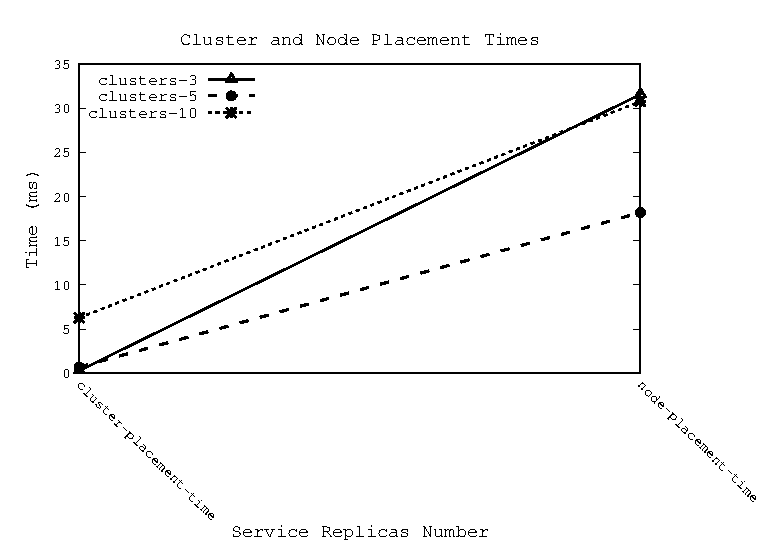
\includegraphics{results/placement-times.eps}
\caption{Cluster and Node Placement Times}\label{fig:placement-times.eps}
\end{figure}

\subsection{}

\begin{lstlisting}[caption={Cluster CPU Utilization}]
Cluster CPU Utilization (%)
replications cluster-1 cluster-2 cluster-3
replica-1 7,00 0,00 0,00
replicas-5 39,00 0,00 0,00
replicas-10 78,00 0,00 0,00
replicas-20 99,40 0,00 56,40
replicas-30 99,60 34,70 99,00
\end{lstlisting}

\begin{figure}[ht]
\centering
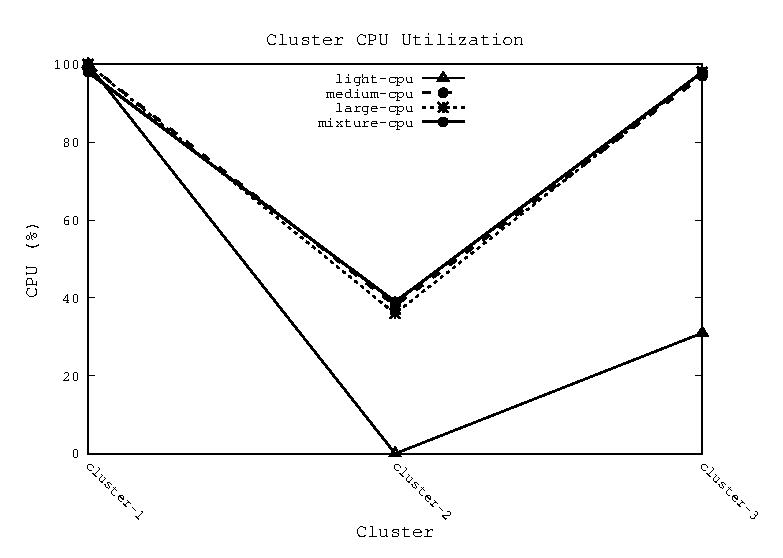
\includegraphics{results/cluster-cpu-utilization.eps}
\caption{Cluster CPU Utilization}\label{fig:cluster-cpu-utilization.eps}
\end{figure}

\subsection{}

\begin{lstlisting}[caption={Cluster Memory Utilization}]
Cluster Memory Utilization (%)
replications cluster-1 cluster-2 cluster-3
replica-1 3,00 0,00 0,00
replicas-5 19,00 0,00 0,00
replicas-10 39,00 0,00 0,00
replicas-20 49,60 0,00 28,00
replicas-30 50,00 17,00 49,30
\end{lstlisting}

\begin{figure}[ht]
\centering
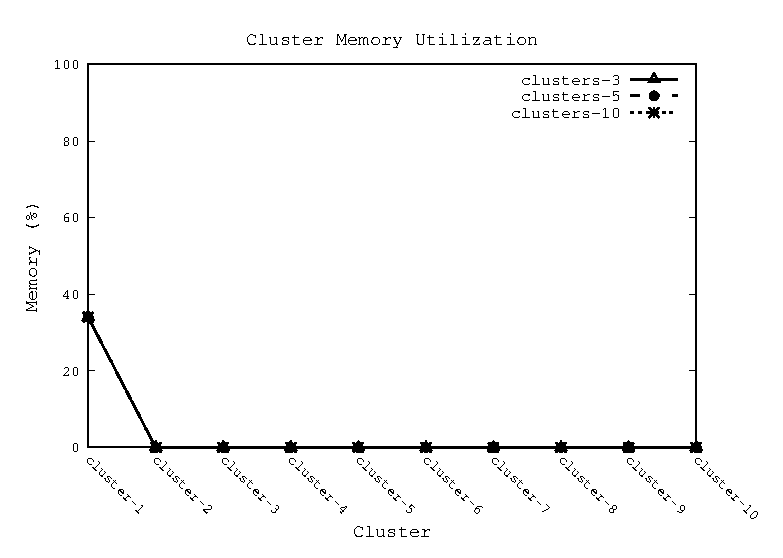
\includegraphics{results/cluster-memory-utilization.eps}
\caption{Cluster Memory Utilization}\label{fig:cluster-memory-utilization.eps}
\end{figure}

\subsection{}

\begin{lstlisting}[caption={Cluster Node Utilization}]
Cluster Node Utilization (%)
replications cluster-1 cluster-2 cluster-3
replica-1 100,00 0,00 0,00
replicas-5 100,00 0,00 0,00
replicas-10 100,00 0,00 0,00
replicas-20 100,00 0,00 100,00
replicas-30 100,00 100,00 100,00
\end{lstlisting}

\begin{figure}[ht]
\centering
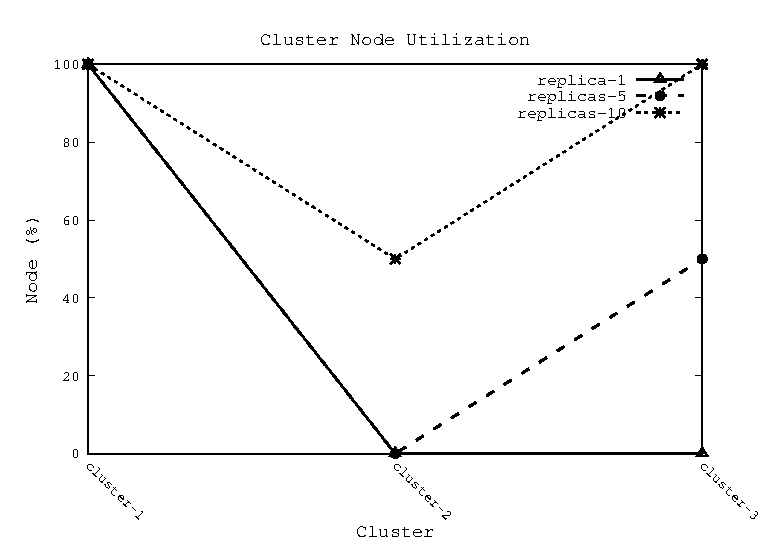
\includegraphics{results/cluster-node-utilization.eps}
\caption{Cluster Node Utilization}\label{fig:cluster-node-utilization.eps}
\end{figure}

\subsection{}

\begin{lstlisting}[caption={Node CPU Utilization}]
Node CPU Utilization (%)
nodes cluster-1-node1 cluster-1-node2 cluster-2-node1 cluster-2-node2 cluster-3-node1 cluster-3-node2
replica-1 7,00 7,00 0,00 0,00 0,00 0,00
replicas-5 39,00 39,00 0,00 0,00 0,00 0,00
replicas-10 78,00 78,00 0,00 0,00 0,00 0,00
replicas-20 99,60 99,00 0,00 0,00 99,20 12,80
replicas-30 99,50 99,70 69,40 0,00 98,40 99,50
\end{lstlisting}

\begin{figure}[ht]
\centering
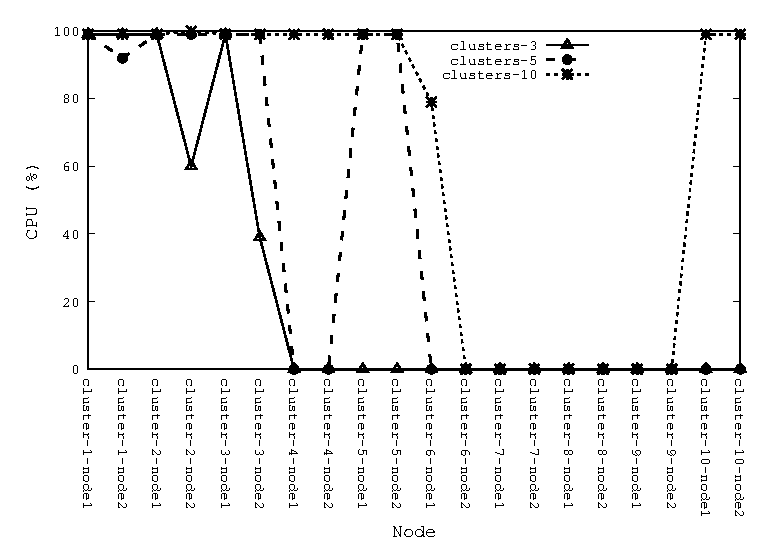
\includegraphics{results/node-cpu-utilization.eps}
\caption{Node CPU Utilization}\label{fig:node-cpu-utilization.eps}
\end{figure}

\subsection{}

\begin{lstlisting}[caption={Node Memory Utilization}]
Node Memory Utilization (%)
nodes cluster-1-node1 cluster-1-node2 cluster-2-node1 cluster-2-node2 cluster-3-node1 cluster-3-node2
replica-1 3,00 3,00 0,00 0,00 0,00 0,00
replicas-5 19,00 19,00 0,00 0,00 0,00 0,00
replicas-10 39,00 39,00 0,00 0,00 0,00 0,00
replicas-20 50,00 49,60 0,00 0,00 50,00 6,40
replicas-30 50,00 50,00 34,70 0,00 49,30 50,00
\end{lstlisting}

\begin{figure}[ht]
\centering
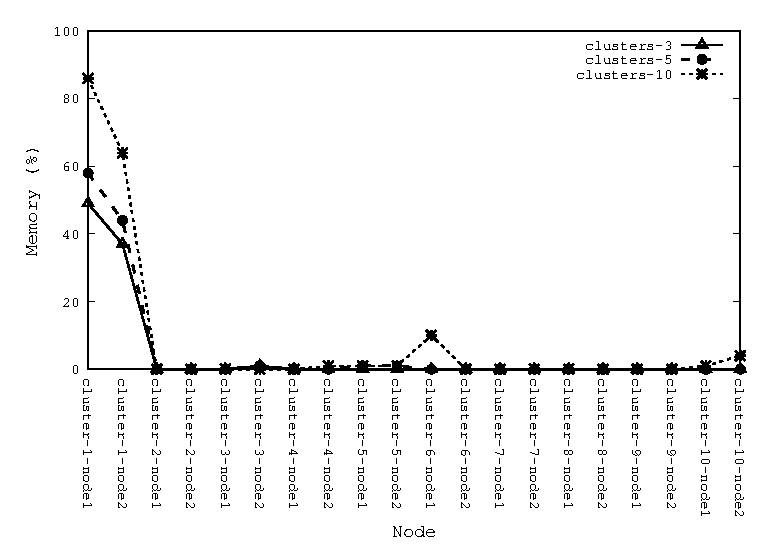
\includegraphics{results/node-memory-utilization.eps}
\caption{Node Memory Utilization}\label{fig:node-memory-utilization.eps}
\end{figure}


\end{document}
